%!TEX root = ../main.tex

\chapter{Introduction}
\label{ch:intro}
%Page budget for Introduction: 3-5 pages.
Distributed database systems in the Blockchain are an emerging technology aiming to provide users with the required tools to perform tasks and computations without an intermediate entity, to build self-trust systems where the rules are agreed upon beforehand and set the basis for a universal ecosystem. Users can then interact democratically and ensure that the committed transactions will be immutable truthful, confident, and non-reTpudiable.
The most famous case of a worldwide distributed blockchain system is Bitcoin. 

By the time this work is written, bitcoin had demonstrated robustness, reliability, and proof that new ways of trust/collaboration can be built on the Internet over 14 years (since its implementation in 2019) to remediate the economic boundaries that banks are still unable to solve.

[CITATION REQUIRED] 


To enable a self trusted system, the Bitcoin standard implemented in its technology a proto-scripting language where all participants agree upon a set of base rules such as:
A maximum capital of 21,000,000 bitcoins will ever exist.
During the first 210,000 blocks, each block produced 50 bitcoins (approximately every 10 minutes).
After the first 210,000 blocks, the number of Bitcoins generated will halve to 25 bitcoins (the number keeps halving approximately every four years), with the last Bitcoin generated somewhere in 2140.
This new economic agreement aims to generate a deflationary economy. The currency's value will likely increase over time (emulating scarce resources). 
The proto scripting language generated two concepts of ecnomic tokenization and usability:

Many projects are emerging from the original idea of Blockchain, specially created to remediate the economic boundaries that banks are still unable to solve. New standards for code as a "proof of trust" created the possibility to develop and compile source code in the blockchain (better known as smart contracts). 

 however, little has been researched so far for its application in the industry, where supply chain and 

  and the basis for different projects 
Industries can nowadays benefit from blockchain systems to record and track data in more trustful ways and allow cooperation. However, the problem of privacy, ownership, and security emerges when trying to implement such systems. In this thesis project, a schema and system design is proposed to record unique ownership of certain assets in the blockchain (datasets ownership) and provide the infrastructure to allow its usage or deny it depending on the agreements of the system through the issuance of NFT's for specific datasets.


Distributed database systems in the Blockchain are an emerging technology aiming to provide users with the required tools to perform tasks and computations without an intermediate entity, to build self-trust systems where the rules are agreed upon beforehand and set the basis for a universal ecosystem. Users can then interact democratically and ensure that the committed transactions will be immutable truthful, confident, and non-repudiable.
The most famous case of a worldwide distributed blockchain system is Bitcoin. 

By the time this work is written, bitcoin had demonstrated robustness, reliability, and proof that new ways of trust/collaboration can be built on the Internet over 14 years (since its implementation in 2019) to remediate the economic boundaries that banks are still unable to solve. \cite{nakamoto2008bitcoin}

To enable a self trusted system, the Bitcoin standard implemented in its technology a proto-scripting language where all participants agree upon a set of base rules such as:
\begin{itemize}
\item A maximum capital of 21,000,000 bitcoins will ever exist. 
\item During the first 210,000 blocks, each block produced 50 bitcoins (approximately every 10 minutes).
\item After the first 210,000 blocks, the number of Bitcoins generated will halve to 25 bitcoins (the number keeps halving approximately every four years), with the last Bitcoin generated somewhere in 2140.
\item This new economic agreement aims to generate a deflationary economy. The currency's value will likely increase over time (emulating scarce resources). 
\end{itemize}

Bitcoin's proto-scripting language generated new ways where economic tokenization \cite{malinova2018tokenomics} and finance and token usability can help implement for the first time trustless systems of worldwide cooperation

Many projects are emerging from the original idea of Blockchain, specially created to remediate the economic boundaries that banks are still unable to solve. New consensus standards in source code to represent a "proof of trust" created the possibility to develop and compile immutable agreements potentially improbable to break when all the parties agree on its contents and liabilities. The term "smart contract" accrued by Nick Szabo in 1997 \cite{szabo1997formalizing}, came to life with the first computer peers joint the Bitcoin Network.

Through this protocols and smart contracts the concepts of digital fungible asset and  non-fungible asset permitted a new way to transact and send value by altering the Blockchain ledger.

Bitcoins are in its essence fungible tokens\footnote{An object is fungible when and if it is identical to others and thus can be replaced without any loss (mutual interchangeability).}, but it also allows since its creation the minting of "Coloured coins, better known as non-fungible tokens (NFT).\footnote{As bitcoins scripting language allows the coding of basic instructions, it is possible to represent asset manipulation through the exchange of assets. This makes possible to create the concept of unicity in a ledger, making a transaction or an asset irrepeatable.}

\section{Background and Motivation}
\label{sec:motivation}
Non-fungibility in the blockchain brings tremendous possibilities to store value and a representation of physical or virtual objects. When the concept was exploited and implemented as a true protocol in the Ethereum Environment, \footnote{Ethereum is another decentralized open source blockchain with smart contract functionality embedded since its conception. Conceived in 2013, its creator extended the potential that Bitcoin had as a decentralized system to enable the generation of digital contracts.} the public realized of the potential the technology could have to generate value over the issuance of public certificates able to be verified by anyone to proof authenticity or ownership for predefined assets. 
\begin{figure}[h]
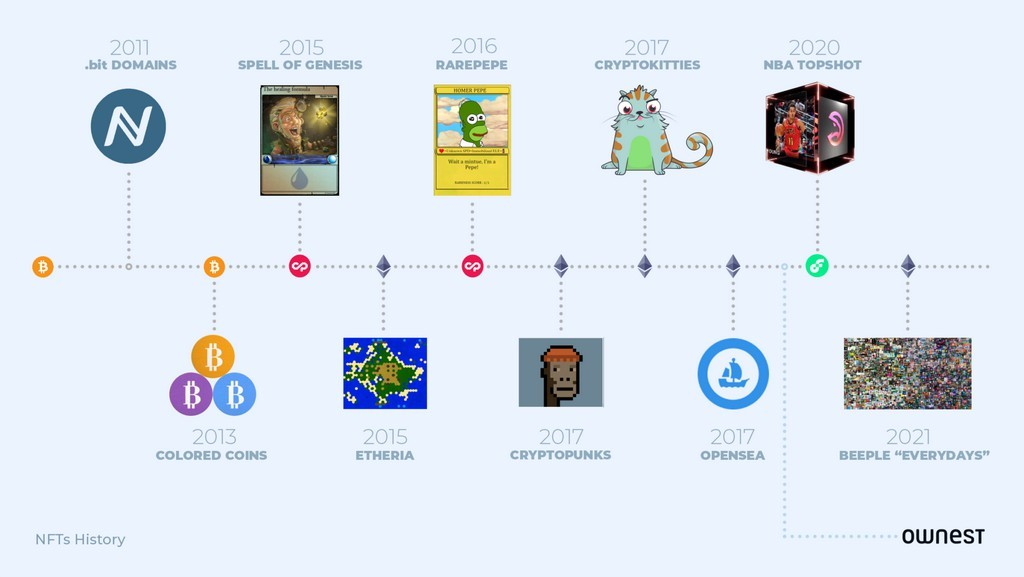
\includegraphics[width=15cm]{img/01-NFT_Timeline.png}
\centering
\caption{NFT Timeline, from the creation of Bitcoin domains, coloured coins to the new Ethereum and Altcoin derivatives  \cite{OwnestNF21:online}}
\end{figure}

Although NFTs have skyrocketed from public Blockchains to demonstrate their potential with digital art (paintings, music, certification of authenticity, among others), little has been researched and implemented in the industry.

Industries can nowadays benefit from blockchain systems to record and track data in more trustful ways and allow inter-entity cooperation. However, the problem of privacy, ownership, and security and finance emerges when trying to implement such systems on a public blockchain. 

In this thesis project, a schema and system design is proposed to record unique ownership of certain assets in the blockchain (datasets ownership) and provide the infrastructure to allow its usage or deny it depending on the agreements of the system through the issuance of NFT's for specific datasets.

\section{Objectives}
\begin{itemize}
    \item Create a permissioned system blockchain with the ability to store Digital Assets through the use and extension of the ERC-721 protocol and expand its potential for file storage, data sharing and distribution.
    \item Use the protocol IPFS to store data and link tis address in the blockchain
    \item Implemente a consensus mechanism that incentivizes the cooperation and participation of different parties with the intention of share, trust, compose and improve data structures and other systems by implementing the blockchain system.
    \item Provide a baseline platform to allow the usage of tokens and promote the fair play in the system
    \item Explor additional consensus mechanism as a reference for future research
    \item Create a system able to represent ownership of certain digital assets through the emission of \ac{NFT}
\item Propose a system to transfer such NFTS between institutions as the equivalent of ownership transfer
\item Link the ownership system with the identity and blockchain databases.
\item Demonstrate that proposed functionality could enable institutions and corporations easy ways to cooperate and compute datasets by using ownership mechanisms

\end{itemize}


\section{Approach and Contributions}

This thesis works uses Hyperlesdger Fabric permissioned Blochcain framework as a base platform to implement an ERC-721 smart contract extension for the creation and certification of digital assets, whic for the aim of this thesesi s represented in data. 
It also implements an distributed data lake infrastructure throuh the usage of a private IPFS network, which allows storage of information in a reliable and trustless mannner. When this data is linked to the ERC-721 smart contract, an NFT asset is created, and single entity properties like ownership, authenticity, transfer, royalties, etc, can be exposed to all its participants.

It demonstrate through the createon of a backend and frontend example applications the potential of its usage through a simulated token minting and data sharing environmnet among different known parties where the unique source of trust is a centrar authority and the previous agreement of the rules (consensus protocol) through which the data can be generated, shared and transfered in the same manner as if a crypto asset was transferred.
\subsection{Implementation}
Since the enviornment has been implementesd using Docker Containers Technology, its scalability and security are granted and can be easily implemented.

\subsection{results}

the results can be visualized in  the following github repository, the program can be downloaded and deployed in any computer system with specifi requirements
\begin{itemize}
    \item ERC-721 protocol creation and extension
    \item Consensus mechanism
    \item Infrastructure and blochcain enviromnent in hyperledger Fabric
    \item REST API in the backend for common collaboration with tthe blockchain
    \item Front wne Web application as a simulation of  work and data generation through the blockchain
    \item Creation of a private IPFS netwrork and data persistance schema for common data sharing
\end{itemize}

\subsection{anaylsys}
A detailed analysis of the systems infrasdtructure and collaboration, the interretation of roles and mechanisms that an organization will play to grant plain participation and collaboration over the blockchain systems in hyperledgher
Data persistance and availability in the IPFS environment,

Generation of a proof of authenticity and non repudiation fo data, consensus protoco, trhough the exploration of the blockchain and closes application system

\begin{itemize}
\item Give a brief summary of your overall approach.
\item Summarize the specific contributions that you made in this thesis (implementation, empirical results, analysis, etc.).
\end{itemize}


\section{Outline}
The thesis projects consists of the following chapters:
\subsection{Chapter 2. Related work}
\subsection{Chapter 3. Approach}
\subsection{Chapter 2. Experimental evaluation}
\subsection{Chapter 2. Token economics}
\subsection{Chapter 3. Fungibility and non fungibilityy}
\subsection{Chapter 4. Fungibility and non fungibilityy}
\subsection{Chapter 5. IPFS as a decentralized File system}
\subsection{Chapter 6. Hyperledger fabric as a permissioned blockchain network}
\subsection{Chapter 7. Implementation of the Digital Asset System }
\subsection{Chapter 8. The consensus protocol }
\subsection{Chapter 9. Proof of ownership }
\subsection{Chapter 10. Simulation and program }
\subsection{Chapter 11. Future work }
\subsection{Chapter 12. Conclusions }
\subsection{Chapter 12.Bibliography }


\begin{itemize}
\item Give an overview of the main points and the structure of your thesis.
\item Examples: ``Chapter 2 covers ...  Chapter 3 describes ...''
\item Show how the different parts (chapters) relate to each other.
\end{itemize}



